\chapter{Methods and techniques}%
\label{ch:methods}

Since the works described in~\cref{ch:paper1,ch:paper2,ch:paper3} consist
of contributions related to the computational elucidation of reaction mechanisms,
this chapter presents an account of the relevant computational methods and
techniques used in the investigations,
with background and context given
for the various topics where appropriate.
A basic background on computational chemistry applied
to mechanistic elucidation is given in~\cref{sec:background-methods}.
Details about the methods used in the development of the \overreact software
package are given in~\cref{sec:overreact-methods}.

\subimport{.}{methods/background}

\section{Chemical reaction mechanisms}

Hypothetical reaction mechanisms consist of
the interpretation of the available data for a chemical reaction
in terms of a model that is self-consistent.
Proposals for reaction mechanisms must be compared
with each other
and with the available experimental data.
Many different hypotheses for the same reaction can exist,
and,
after pruning the ones in disagreement with the available data,
it is still possible to have several different plausible models at hand.
Computational modelling of chemical reactions
provides one with a way of
formulating,
analyzing and
comparing hypotheses to each other,
to the literature and to the available experimental data.
This way,
one is able to come up with a ``most probable'' one.

\subsection{Bell-Evans-Polanyi principle}

The Bell-Evans-Polanyi (BEP) principle is a fundamental principle in the study
of chemical reactions.
It states that the more exothermic reactions usually have to overcome lower
reaction barriers and are therefore faster.

% TODO: equations,
% main features,
% scheme,
% missing!

It is customary to successfully extend this concept to exergonic reactions.
But since the largest contribution is the electronic energy,
it is reasonably
safe to apply the BEP principle (and Hammer's postulate,
as we will see later)
using electronic energies in the context of quantum chemistry calculations.

% TODO
IN THE NOTES.\@
CITATION.\@

\subsection{Hammond's postulate}

% TODO:
THIS IS CITED IN THE INTRO AS WELL

IN THE NOTES.\@
CITATION.\@

\section{Intramolecular and substitutional effects:
  a key step to understand enzyme-like catalysis}

Despite the great advancements in the developments of artificial enzymes~\cite{Breslow_1995},
the synthetic reproduction of the reaction rate accelerations attained by
natural enzymes is far from being reached.
To get there,
we will need a more detailed comprehension of the ways enzymes
work at the molecular level~\cite{Catalysis_in_Chemistry_and_Enzymology}.
Much effort has been put in this direction,
with at least six Nobel Prizes
awarded in this and related areas~\cite{Nobel_1929,Nobel_1946,Nobel_1957,Nobel_1975,Nobel_1997,Nobel_2013}.
These progresses show that the main source of acceleration in
enzymatic reactions is to be found in the events that accompany the
enzyme-substrate complex formation that leads to bond breaking and
formation~\cite{Catalysis_in_Chemistry_and_Enzymology}.
These events induce conformational changes in both substrate and enzyme,
which
enhances the interactions in the active site~\cite{Fischer_1890,Fischer_1894,Koshland_1958,Dafforn_1971,Kirby_1996}.
PICTURES OF REPRESENTATIVE SCHEMES!\@
As a result,
substrate active centers adequately orient themselves towards
their counterparts in the active site,
which leads to
i.\ a decrease in stability of the ground state (if compared with the
free substrate state),
ii.\ a lowering of the transition state energy (if compared with the
non-catalyzed reaction),
iii.\ energy relaxation through the formation of intermediates and
products.

These driving forces are also found in intramolecular reactions (\cref{fig:reacoes-intramoleculares}).
%
\begin{figure}[hbtp]
	\centering
	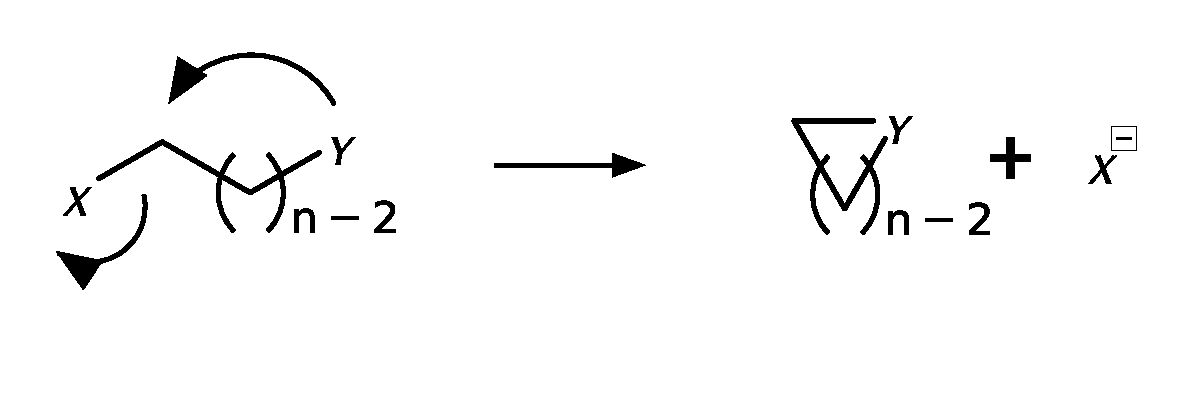
\includegraphics[width=.6\textwidth]{figures/reacao-intramolecular}
	\caption[Typical scheme of an intramolecular reactions]{
		Reaction scheme of a typical intramolecular reaction,
		whose products or
		intermediates are often cycles.
		Smaller rings ($n \le 4 $)
		tend to be disfavored by enthalpy,
		while larger rings ($n \ge 7 $)
		have less probable formation due to entropy.}%
	\label{fig:reacoes-intramoleculares}
\end{figure}
%
In fact,
the similarities between monomolecular enzymatic processes and
intramolecular reactions have been already recognized~\cite{Nilsson_1933,Bruice_1960b,Jung_1990}.
Despite the limitations of using intramolecular reactions as a model for
enzymatic reactions,
it is natural to suppose that the detailed understanding
of enzyme catalysis has,
as a prerequisite,
the ability to understand the
related processes in simpler systems.~\cite{Kirby_1972}.

We have studied some of these effects.
WHICH ONES?\@

% TODO: concatenate the results with those remarks.
% It's OK not to have it all!
% PAPER 1 => is peptide-like/enzyme-like? is intramolecular/substitutional?
% PAPER 2 => is peptide-like/enzyme-like? is intramolecular/substitutional?
% PAPER 3 => is peptide-like/enzyme-like? is intramolecular/substitutional?
% => \emph{\ce{N}}-alkyl substituted maleamic acids
Particular details concerning the intramolecular effects of geminal and
vicinal disubstitutions can be found in~\cref{ch:gem-vic-disubstitions}.

\subimport{.}{methods/overreact}

% TODO: things from the quali
% Mecanismos foram validados com base na concordância relativa aos respectivos resultados experimentais~\cite{Kirby_1972,Jung_2005}.
% A termoquímica relevante foi calculada à condição de temperatura e pressão ambientes (298.15~K e 1~atm).
% Determinações de \emph{pKa} dos compostos estudados também foram realizadas com
% relação ao ácido acético,
% de acordo com o esquema de
% \citeauthor{Ding_2009}~\cite{Ding_2009} (\cref{sec:pka}).

% Cálculos foram realizados com o programa Gaussian~09C.01~\cite{g09} e com o funcional da densidade
% % PBE0~\cite{Perdew_1996,Perdew_1997,Ernzerhof_1999,Adamo_1999}
% \emph{wB97XD}~\cite{Chai_2008a,Chai_2008b} (\cref{sec:funcionais}),
% que foi
% utilizado em conjunto com funções de base de Pople de qualidade triplo-$\zeta$
% com funções difusas e polarizações em todos os átomos
% (\emph{6--311++G**}~\cite{Ditchfield_1971,Hehre_1972,Hariharan_1973,Hariharan_1974,Gordon_1980,Francl_1982,Clark_1983,Frisch_1984,Binning_1990,Blaudeau_1997,Rassolov_1998,Rassolov_2001},~\cref{sec:basis-functions}).
% Todos os cálculos levaram em consideração efeitos de solvatação aquosa através
% do uso do \emph{SMD},
% desenvolvido por \citeauthor{Marenich_2009} (\cref{sec:implicit-solvation}).
% De forma a se investigar o efeito da geometria do estado fundamental,
% uma
% análise conformacional dos compostos foi empregada,
% usando o programa Open
% Babel 2.4.1~\cite{O_Boyle_2011} com o \emph{PM7} (MOPAC2016~\cite{MOPAC},~\cref{sec:conformational-analysis}).

% Estruturas eletrônicas dos compostos serão estudadas à luz dos \emph{NBO}
% (\cref{sec:nbos}).

% em particular para se correlacionar o efeito cinético da substituição
% \begin{enumerate*}[label=(\roman*)]
%   \item com eventuais flutuações de hibridização dos carbonos da ponte~\cite{Bent_1961} e
%   \item com a magnitude da repulsão estérica entre substituintes e grupos reativos.
% \end{enumerate*}

% Para tanto será utilizado o programa NBO~5.9~\cite{NBO5.9} acoplado com o programa Gaussian~09C.01~\cite{g09}.
